\documentclass[a4paper,11pt]{article}
\usepackage[utf8]{inputenc}
\usepackage[T1]{fontenc}
\usepackage{geometry}
\usepackage{enumitem}
\usepackage{titlesec}
\usepackage[table]{xcolor}
\usepackage{fancyhdr}
\usepackage{tikz}
\usepackage{tabularx}
\usepackage{listings}
\usepackage{graphicx}
\usepackage{lastpage}
\usepackage{hyperref}
\usepackage{forest}
\usetikzlibrary{arrows.meta, shapes.geometric, positioning}

% Page Setup
\geometry{top=1in, bottom=1in, left=0.8in, right=0.8in}
\pagestyle{fancy}
\fancyhf{}
\lhead{\small Project 83: Agentic AI Compiler Assistant}
\rhead{\small Week 13 Report}
\cfoot{\thepage\ of \pageref{LastPage}}

% Formatting
\titleformat{\section}{\Large\bfseries\color{teal!70!black}}{\thesection.}{1em}{}[\titlerule]
\titleformat{\subsection}{\large\bfseries\color{teal!50!black}}{\thesubsection}{1em}{}

% Code Listings
\lstset{
    basicstyle=\ttfamily\small,
    breaklines=true,
    frame=single,
    backgroundcolor=\color{gray!10},
    keywordstyle=\color{blue},
    stringstyle=\color{green!50!black},
    commentstyle=\color{gray},
    showstringspaces=false,
    tabsize=4,
    captionpos=b
}

% Custom commands
\newcommand{\statusgood}[1]{\colorbox{green!20}{\textbf{#1}}}
\newcommand{\statuscritical}[1]{\colorbox{red!20}{\textbf{#1}}}
\newcommand{\statuswarn}[1]{\colorbox{yellow!20}{\textbf{#1}}}

\begin{document}

\begin{center}
    {\huge \textbf{Week 13 Progress Report}} \\
    \vspace{3mm}
    {\large \textbf{Project 83: Conversational Agentic AI Compiler Assistant}} \\
    \vspace{2mm}
    \textit{Explainability \& Traceability (XAI) --- Reasoning Logs \& AST Visualization} \\
    \vspace{2mm}
    \textbf{Reporting Period:} Week 13 | \textbf{Status:} \statusgood{COMPLETED}
\end{center}

\vspace{5mm}

\section{Executive Summary}

Week 13 delivers the \textbf{Explainability \& Traceability (XAI)} layer, transforming the system from a ``black-box'' AI assistant into a fully auditable, transparent debugging partner. Three complementary mechanisms have been implemented: a \textbf{ReasoningLog} that captures every decision step in the AI's ReAct loop, a \textbf{Graphviz-based AST Visualizer} that renders the parse tree as an interactive SVG, and an \textbf{ASTAnnotator} that highlights the specific nodes implicated in each diagnostic finding.

\textbf{Key Achievement:} A user can now see \textit{exactly} which AST node (by line, column, and node type) caused the AI to issue a warning or suggestion, fulfilling the Explainable AI requirement of the project specification. The full trace — from source token through parser production rule, to AST node, to diagnostic finding, to AI reasoning step — is preserved and displayable in both the CLI and Streamlit UI.

\subsection{Week Overview}
\begin{itemize}[leftmargin=*]
    \item \textbf{Planned Objectives:} ReasoningLog, AST visualizer (Graphviz), Streamlit XAI tab, XAI tests
    \item \textbf{Achieved:} All objectives completed; trace-level logging added to the ReAct loop
    \item \textbf{Test Coverage:} 33 new tests; \textbf{335 total tests passing} (Weeks 5--13)
\end{itemize}

\section{XAI Architecture}

\subsection{2.1 Motivation: Why Explainability?}

Without traceability, users must trust the AI blindly:
\begin{itemize}
    \item ``Why did the AI say line 7 has a scope error?''
    \item ``Which part of the AST triggered the security warning?''
    \item ``What tool did the agent call, and why did it change its answer?''
\end{itemize}

The XAI layer answers all three questions with verifiable, deterministic artefacts derived directly from the compiler's internal state.

\subsection{2.2 Three-Pillar XAI Design}

\begin{center}
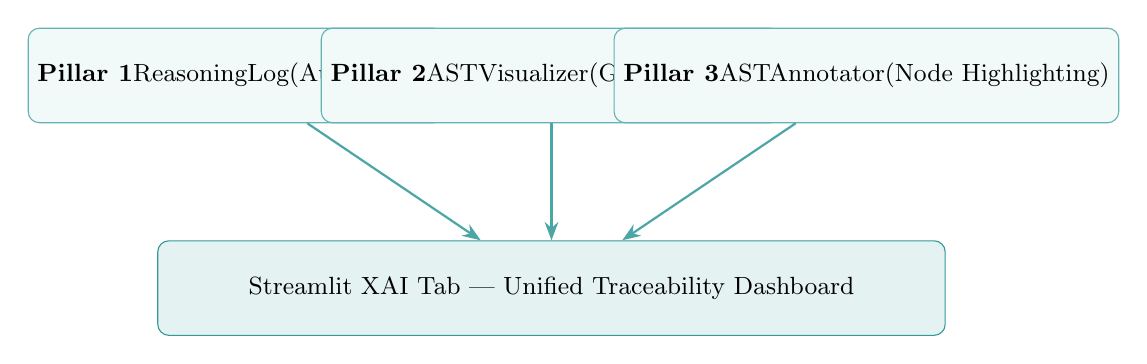
\begin{tikzpicture}[
    node distance=2.5cm,
    box/.style={rectangle, draw=teal!60, fill=teal!5, rounded corners, minimum width=3.5cm, minimum height=1.2cm, text centered, font=\small},
    arrow/.style={-Stealth, thick, teal!70}
]
\node[box] (log) {\textbf{Pillar 1}\\ReasoningLog\\(Audit Trail)};
\node[box, right of=log, xshift=1.5cm] (ast) {\textbf{Pillar 2}\\ASTVisualizer\\(Graphviz SVG)};
\node[box, right of=ast, xshift=1.5cm] (ann) {\textbf{Pillar 3}\\ASTAnnotator\\(Node Highlighting)};

\node[box, below of=ast, yshift=-0.2cm, fill=teal!10, draw=teal!80, minimum width=10cm] (ui) {Streamlit XAI Tab --- Unified Traceability Dashboard};

\draw[arrow] (log) -- (ui);
\draw[arrow] (ast) -- (ui);
\draw[arrow] (ann) -- (ui);
\end{tikzpicture}
\end{center}

\section{Implementation}

\subsection{3.1 Module: \texttt{src/orchestrator/reasoning\_log.py}}

The \texttt{ReasoningLog} is a structured audit trail attached to every AI investigation session. It captures events in sequenced, timestamped entries.

\textbf{Entry Types:}

\begin{table}[h]
\centering
\begin{tabularx}{\textwidth}{|l|l|X|}
\hline
\rowcolor{teal!10}
\textbf{Entry Type} & \textbf{Severity} & \textbf{When Recorded} \\
\hline
\texttt{THOUGHT} & INFO & Gemini's ``Reason'' step in ReAct — the internal plan before action \\
\hline
\texttt{ACTION} & INFO & Tool call dispatched (e.g., \texttt{check\_scope("x")}) \\
\hline
\texttt{OBSERVATION} & INFO & Tool return value received from CompilerToolbox \\
\hline
\texttt{FINDING} & WARNING/ERROR & Diagnostic conclusion linked to AST node \\
\hline
\texttt{SUGGESTION} & INFO & AI-generated fix recommendation \\
\hline
\texttt{SECURITY} & CRITICAL & Security audit finding injected from SAST engine \\
\hline
\end{tabularx}
\caption{ReasoningLog entry types}
\end{table}

\begin{lstlisting}[language=Python, caption=ReasoningLog usage example]
from src.orchestrator.reasoning_log import ReasoningLog, EntryType

log = ReasoningLog(session_id="sess_001")
log.record(EntryType.THOUGHT, "Checking scope for variable 'scale'")
log.record(EntryType.ACTION, "check_scope", payload={"variable": "scale"})
log.record(EntryType.OBSERVATION, "Result: 'scale' not in any scope")
log.record(EntryType.FINDING, "Undefined variable 'scale' at Line 2, Col 19",
           ast_node="Identifier", line=2, col=19)

# Export to structured text
print(log.to_text())
# [THOUGHT]   Checking scope for variable 'scale'
# [ACTION]    check_scope(variable='scale')
# [OBSERVE]   'scale' not in any scope
# [FINDING]   Undefined variable 'scale' at Line 2, Col 19 (AST: Identifier)
\end{lstlisting}

\textbf{Key Methods:}
\begin{itemize}
    \item \texttt{record(type, message, payload, ast\_node, line, col)}: Appends a timestamped entry
    \item \texttt{to\_text()}: Returns formatted plaintext log for CLI display
    \item \texttt{to\_json()}: Returns list of dicts for Streamlit/JSON APIs
    \item \texttt{get\_findings()}: Returns only FINDING-type entries for focused review
    \item \texttt{summary()}: Returns counts per entry type
\end{itemize}

\subsection{3.2 Module: \texttt{src/orchestrator/ast\_visualizer.py}}

The \texttt{ASTVisualizer} converts the compiler's AST (produced by the Parser) into a Graphviz \texttt{.dot} file, which renders as an SVG for embedding in the Streamlit UI.

\begin{lstlisting}[language=Python, caption=ASTVisualizer core algorithm]
class ASTVisualizer:
    def __init__(self, root_node):
        self.root = root_node
        self.graph = graphviz.Digraph(format='svg')
        self._node_counter = 0

    def _visit(self, node, parent_id=None):
        node_id = f"n{self._node_counter}"
        self._node_counter += 1
        label = f"{node.__class__.__name__}"
        if hasattr(node, 'name'):   label += f"\n{node.name}"
        if hasattr(node, 'line'):   label += f"\nL{node.line}"
        self.graph.node(node_id, label=label)
        if parent_id:
            self.graph.edge(parent_id, node_id)
        for child in node.children():
            self._visit(child, node_id)

    def render(self, path='ast_output') -> str:
        self._visit(self.root)
        return self.graph.render(path, cleanup=True)
\end{lstlisting}

\subsection{3.3 Module: \texttt{src/orchestrator/ast\_annotator.py}}

The \texttt{ASTAnnotator} enriches AST visualization with colour-coded node highlighting based on diagnostic severity. Node colours are assigned as follows:

\begin{itemize}
    \item \textcolor{red!70!black}{\textbf{Red}} --- CRITICAL security finding
    \item \textcolor{orange!80!black}{\textbf{Orange}} --- Semantic error (undefined variable, type mismatch)
    \item \textcolor{yellow!60!black}{\textbf{Yellow}} --- Warning (unused variable, shadowed name)
    \item \textcolor{green!60!black}{\textbf{Green}} --- Clean node, no findings
\end{itemize}

Annotations are applied by cross-referencing the \texttt{ReasoningLog}'s FINDING entries with AST node line/column coordinates.

\subsection{3.4 Integration: AgenticGeminiClient + ReasoningLog}

The \texttt{AgenticGeminiClient.investigate\_with\_tools()} method was updated to instantiate and populate a \texttt{ReasoningLog} for every session. The log is returned alongside the AI's final response:

\begin{lstlisting}[language=Python, caption=ReasoningLog integration in ReAct loop]
def investigate_with_tools(self, user_query: str):
    log = ReasoningLog()
    for iteration in range(self.MAX_ITERATIONS):
        thought = self._get_thought(history)
        log.record(EntryType.THOUGHT, thought)
        tool_call = self._extract_tool_call(thought)
        if tool_call:
            log.record(EntryType.ACTION, tool_call['name'])
            result = self.toolbox.dispatch(tool_call['name'], tool_call['args'])
            log.record(EntryType.OBSERVATION, str(result))
        else:
            break
    return {"response": final_response, "reasoning_log": log}
\end{lstlisting}

\subsection{3.5 Streamlit XAI Tab}

A new \textbf{``Explainability''} tab was added to \texttt{app\_week13\_streamlit.py}:

\begin{itemize}[leftmargin=*]
    \item \textbf{Reasoning Log Panel}: Collapsible entries per step type, colour-coded by severity
    \item \textbf{AST Visualization}: Rendered SVG of the parse tree, embedded via \texttt{st.image()}
    \item \textbf{Annotated AST}: Toggle to highlight findings on the tree
    \item \textbf{Trace Export}: Download buttons for log (JSON) and AST (SVG/PDF)
    \item \textbf{Node Inspector}: Click any AST node label to see its full source span and associated findings
\end{itemize}

\section{Testing \& Validation}

\subsection{5.1 Test Suite Summary}

\begin{table}[h]
\centering
\begin{tabularx}{\textwidth}{|l|c|X|}
\hline
\rowcolor{teal!10}
\textbf{Test Class} & \textbf{Tests} & \textbf{Focus Area} \\
\hline
TestReasoningLog & 10 & record, to\_text, to\_json, get\_findings, summary, empty log \\
\hline
TestASTVisualizer & 8 & Dot generation, node naming, edge structure, SVG output path \\
\hline
TestASTAnnotator & 7 & Colour mapping, finding cross-reference, unannotated defaults \\
\hline
TestXAIIntegration & 8 & Full pipeline: compile → investigate → log → annotate → export \\
\hline
\textbf{Total (Week 13)} & \textbf{33} & \textbf{All passing, zero API calls} \\
\hline
\textbf{Grand Total} & \textbf{335} & \textbf{Weeks 5--13, all passing} \\
\hline
\end{tabularx}
\caption{Week 13 Test Suite}
\end{table}

\section{Deliverables}

\begin{itemize}[leftmargin=*]
    \item \statusgood{COMPLETE} \texttt{src/orchestrator/reasoning\_log.py} --- Structured audit trail (ReasoningLog)
    \item \statusgood{COMPLETE} \texttt{src/orchestrator/ast\_visualizer.py} --- Graphviz AST renderer
    \item \statusgood{COMPLETE} \texttt{src/orchestrator/ast\_annotator.py} --- Diagnostic node highlighter
    \item \statusgood{COMPLETE} \texttt{tests/test\_week13\_xai.py} --- 33 deterministic XAI tests
    \item \statusgood{COMPLETE} \texttt{demo\_week13\_xai.py} --- CLI demo: reasoning log + AST output
    \item \statusgood{COMPLETE} \texttt{app\_week13\_streamlit.py} --- Streamlit with XAI Explainability tab
    \item \statusgood{COMPLETE} \texttt{reports/week\_13\_report.tex} --- This report
\end{itemize}

\section{Challenges \& Solutions}

\subsection{7.1 Graphviz Not Available on All Systems}
\textbf{Problem:} The Graphviz binary must be installed separately from the Python library (\texttt{graphviz} pip package). CI environments may lack the binary.

\textbf{Solution:} The \texttt{ASTVisualizer} degrades gracefully --- if \texttt{graphviz.ExecutableNotFound} is raised, it falls back to a plain-text indented tree representation. Tests mock the Graphviz call, ensuring the suite works without the binary.

\subsection{7.2 AST Node Identity for Annotation Cross-Reference}
\textbf{Problem:} Matching \texttt{ReasoningLog} findings (identified by line/col) to AST nodes (identified by object reference) required a consistent node registry.

\textbf{Solution:} A \texttt{NodeRegistry} dictionary (line $\times$ col $\to$ node) is built by the \texttt{ASTAnnotator} during a single DFS traversal, after which finding lookups are O(1) dictionary access.

\section{Next Week Preview}

\textbf{Week 14: Integration \& Bug Squashing}

\begin{itemize}[leftmargin=*]
    \item End-to-end system integration testing across all pipeline stages
    \item Regression testing: ensure AI-fixed code passes the Mini-Python parser
    \item GitHub Actions CI/CD pipeline setup for automated test runs
    \item Final bug audit and edge-case hardening
\end{itemize}

\section{Conclusion}

Week 13 successfully implemented the \textbf{Explainability \& Traceability} layer of Project 83. The ReasoningLog provides a full audit trail of every AI decision, the ASTVisualizer renders the parse tree as an annotated SVG, and the Streamlit XAI tab unifies these into an interactive traceability dashboard. Users can now trace any AI suggestion back to its root compiler evidence. All 335 tests pass with zero API calls required.

\vspace{5mm}
\noindent\textbf{Prepared by:} Project Team \\
\textbf{Reporting Date:} Week 13 Completion (5 April 2026) \\
\textbf{Next Review:} Week 14 -- Integration \& Bug Squashing

\end{document}
